% !TEX TS-program = pdflatex
% !TEX encoding = UTF-8 Unicode

% This is a simple template for a LaTeX document using the "article" class.
% See "book", "report", "letter" for other types of document.

\documentclass[11pt]{article} % use larger type; default would be 10pt

\usepackage[utf8]{inputenc} % set input encoding (not needed with XeLaTeX)
\usepackage{hyperref}
%%% Examples of Article customizations
% These packages are optional, depending whether you want the features they provide.
% See the LaTeX Companion or other references for full information.

%%% PAGE DIMENSIONS
\usepackage{geometry} % to change the page dimensions
\usepackage{algorithm2e}
\geometry{a4paper} % or letterpaper (US) or a5paper or....
% \geometry{margin=2in} % for example, change the margins to 2 inches all round
% \geometry{landscape} % set up the page for landscape
%   read geometry.pdf for detailed page layout information

\usepackage{graphicx} % support the \includegraphics command and options

% \usepackage[parfill]{parskip} % Activate to begin paragraphs with an empty line rather than an indent

%%% PACKAGES
\usepackage{booktabs} % for much better looking tables
\usepackage{array} % for better arrays (eg matrices) in maths
\usepackage{paralist} % very flexible & customisable lists (eg. enumerate/itemize, etc.)
\usepackage{verbatim} % adds environment for commenting out blocks of text & for better verbatim
\usepackage{subfig} % make it possible to include more than one captioned figure/table in a single float
% These packages are all incorporated in the memoir class to one degree or another...

%%% HEADERS & FOOTERS
\usepackage{fancyhdr} % This should be set AFTER setting up the page geometry
\pagestyle{fancy} % options: empty , plain , fancy
\renewcommand{\headrulewidth}{0pt} % customise the layout...
\lhead{}\chead{}\rhead{}
\lfoot{}\cfoot{\thepage}\rfoot{}

%%% SECTION TITLE APPEARANCE
\usepackage{sectsty}
\allsectionsfont{\sffamily\mdseries\upshape} % (See the fntguide.pdf for font help)
% (This matches ConTeXt defaults)

%%% ToC (table of contents) APPEARANCE
\usepackage[nottoc,notlof,notlot]{tocbibind} % Put the bibliography in the ToC
\usepackage[titles,subfigure]{tocloft} % Alter the style of the Table of Contents
\renewcommand{\cftsecfont}{\rmfamily\mdseries\upshape}
\renewcommand{\cftsecpagefont}{\rmfamily\mdseries\upshape} % No bold!

%%% END Article customizations

%%% The "real" document content comes below...

\title{Relatório do projeto de Geometria Computacional\\Locomoção de robôs utilizando grafos de visibilidade}
\author{Igor dos Santos Montagner}
%\date{} % Activate to display a given date or no date (if empty),
         % otherwise the current date is printed 

\begin{document}
\maketitle

\section{Motivação}
O algoritmo implementado foi o descrito no capítulo 15 do livro "Computational Geometry: Algorithms and Applications", de Berg, van Kreveld, Overmars e Schwarzkopf, que resolve o problema da busca pelo melhor caminho entre dois pontos em um mundo que contém obstáculos poligonais.

A motivação do algoritmo é resolver o problema da locomoção de robôs de maneira ótima: dados uma origem, um destino e uma série de obstáculos poligonais, qual o caminho mais curto entre os dois pontos sem que o robô esbarre em algum objeto? O algoritmo explicado funciona para robôs "pontuais", porém é explicada a generalização para um robô que translada, mas não rotaciona. Nos casos mais gerais outras medidas podem ser usadas além do caminho mais curto, como número de rotações necessárias no caminho ou caminho com menor número de arestas.

\section{Algoritmo}

Dados os pontos $s$, $f$ e um conjunto de polígonos $S$, desejamos encontrar o menor caminho de $s$ até $f$ que não intersecta em nenhum obstáculo de $S$. É provado que o caminho mais curto desviando dos obstáculos é composto somente por segmentos de reta que possuem como extremidades ou vértices de um mesmo polígono ou vértices de polígonos diferentes ou os pontos iniciais e finais. Deste modo, é necessário saber, dado um ponto $p$, quais pontos são visíveis a partir dele, ou seja, quais segmentos de reta $\overline{pw}$, para todo vértice $w \in \{s, f\} \cup \{S\}$, não intersectam com nenhum obstáculo em $S$. O algoritmo é composto de duas partes: determinação do \emph{grafo de visibilidade}, que representa os caminhos visíveis entre pontos iniciais e os obstáculos, e a busca pelo menor caminho dentro deste grafo.

\subsection{Grafo de visibilidade}

O \emph{grafo de visibilidade} tem como vértices os vértices dos obstáculos poligonais mais os pontos iniciais e finais. A aresta $(i, j)$ existe no grafo se o segmento $i,j$ não intercepta nenhum obstáculo poligonal, ou seja, se o ponto $i$ é visível a partir do ponto $j$. 

A partir disto, em cada vértice é feita uma linha de varredura radial no sentido anti-horário que utiliza uma árvore binária balanceada para guardar as arestas que intersectam a linha de varredura no momento atual. Se um vértice $w$ é visível, então o segmento $v,w$ não cruza com nenhuma aresta na linha de varredura. 

O algoritmo é o seguinte:

\begin{algorithm}
\SetKwInOut{Input}{input}
\Input{Obstáculos poligonais P, pontos start e end}
Inicialize um grafo G = (V, E) com os vértices de $P\cup\{start,end\}$ e $E = \emptyset$;
\ForEach{vértice $v$ em $P\cup\{start,end\}$} {
	$W \leftarrow VISIBLE(v, P)$;

	\ForEach{vértice $w$ em $W$} {		
		Adicione a aresta $(v, w)$ a G.
	}
}
\Return{G}
\caption{VISIBILITY$\_$GRAPH}
\end{algorithm}

\begin{algorithm}
\SetKwInOut{Input}{input}
\Input{vértice v, conjunto de obstáculos poligonais P}
Ordene os vértices de acordo com o ângulo que formam com a linha paralela ao eixo X que passa por v. Em caso de empate, vértices mais próximos são considerados "menores". Seja $w_1 \dots w_n$ esta lista ordenada.

Seja $\rho$ uma semi reta paralela ao eixo x positivo que tem início em $v$. Adicione as arestas que intersectam $\rho$ a uma árvore binária balanceada $\tau$, ordenando-as por distância até $v$.

$W \leftarrow \emptyset$

\For{$i \leftarrow 1 \dots n$} {
	\If{$w_i$ for visível a partir de $v$} {
		Adicione $w_i$ a $W$.
	}
	Adicione a $\tau$ as arestas incidentes a $w_i$ que estejam a esquerda da linha de varredura.

	Remova de $\tau$ as arestas incidentes a $w_i$ que estejam a direita da linha de varredura.
}
\Return{W}
\caption{VISIBILE}
\end{algorithm}

\subsubsection{Determinação de visibilidade de um ponto}

Um ponto $q$ é visível a partir de outro ponto $p$ se o segmento $\overline{pq}$ não intersecta nenhuma aresta em $\tau$ e, se ambos pertencem ao mesmo polígono, se o segmento $pq$ não intersecta o interior do polígono. 

Para verificar se um ponto qualquer é visível a partir de outro é necessário verificar a interseção com todos os obstáculos, porém como faremos isto para todos os pontos podemos conseguir um algoritmo melhor. Uma linha de varredura radial é utilizada para ser possível saber se um ponto é visível a partir de outro em tempo $O(lg n)$, dado que a utilizemos para analisar todos os pontos em tempo total $O(n lg n)$.

A linha de varredura  guarda as arestas que a intersectam a no momento, logo se um ponto está a esquerda da aresta mais próxima, então ele é visível, do contrário ele não é visível. Se guardarmos o estado em uma árvore binária balanceada, a aresta mais próxima de $p$ está na folha mais a esquerda da árvore. Deste modo, podemos verificar se um ponto cruza as arestas da linha de varredura em tempo $O(lg n)$.

Se ambos os pontos estão no mesmo polígono e o segmento não intersecta nenhuma aresta, então é possível verificar se o segmento intersecta o polígono verificando se o ponto $p$ está no cone formado pelos vértices ($prev(q)$, $q$, $next(q)$), uma operação que leva tempo constante.

\subsection{Busca pelo menor caminho}

A busca pelo menor caminho no grafo é feita utilizando o algoritmo de Dijkstra. No caso do caminho com menor distância, os pesos nas arestas são a distância euclidiana entre suas duas extremidades. A fila de prioridade utilizada foi um Min-Heap.

\subsection{Complexidade}

A complexidade final do algoritmo é $O(n^2 lg n)$ se implementado com as estruturas de dados propostas no livro. Como a implementação que fiz não utilizou uma árvore binária balanceada, a complexidade final é $O(n^3)$.

\section{Implementação}

O algoritmo foi implementado para o robô pontual e atualmente só funciona bem para polígonos convexos. Em polígonos côncavos, o passo de decidir se dois vértices do mesmo polígono são visíveis fica mais complicado e ainda não implementei a solução correta.

\subsection{Instruções de uso}

O projeto foi implementado utilizando  \href{http://processingjs.org/}{ProcessingJS}, uma implementação da linguagem Processing que utiliza HTML5 para fazer visualização e gráficos interativos na web. Deste modo, somente os navegadores mais "modernos" são capazes de mostrar o projeto corretamente. As versões mais recentes do Firefox e do Chrome são capazes de executar o projeto sem erros. Para executar a versão entregue, é necessário abrir o arquivo index.html usando o Firefox. É recomendado visualizar o projeto em \href{http://vision.ime.usp.br/~igor/geocomp}{meu site na Vision}.

O projeto é capaz de guardar e carregar as simulações feitas em um computador. Para guardar uma simulação basta apertar o botão "Save" e escolher um nome para a simulação. Para carregar uma simulação basta apertar o botão "Load" e clicar na simulação escolhida. As simulações são salvas somente no browser utilizado no momento. Para exportar as simulações salvas, aperte o botão "Export" e copie o texto. Para importar o ambiente em outro browser, aperte "Import" e cole o texto copiado anteriormente.

Para criar uma nova simulação é necessário:
\begin{enumerate}
	\item Criar os obstáculos poligonais;
	\item Definir um ponto inicial;
	\item Definir um ponto final.
\end{enumerate}

Para criar um obstáculo poligonal, basta clicar na área de simulação no local aonde devem ser posicionados os vértices. Ao completar um polígono aperte "Complete Polygon". A partir deste momento pode-se adicionar vértices a um novo polígono.

Para definir os pontos iniciais e finais, clique no botão correspondente e clique na área de simulação para definir o local do ponto.

\subsection{Legenda}


A simulação possui duas partes: determinação do grafo de visibilidade e algoritmo de Dijkstra.

Durante a determinação do grafo de visibilidade, a linha verde representa a linha de varredura (os extremos do segmento atual são os bolinhas verdes) e as arestas vermelhas são as arestas que atualmente cruzam com a linha de varredura e estão no conjunto $\tau$. Durante a determinação dos vértices visíveis a partir de um ponto $p$, quando a linha de varredura muda de vértice, existe um pequeno intervalo em que podemos ver o estado antes e depois da atualização de $\tau$. Se o segmento não cruzou nenhuma aresta em $\tau$, ele é adicionado ao grafo e é pintado de amarelo.

\begin{figure}[!htp]
	\begin{center}
		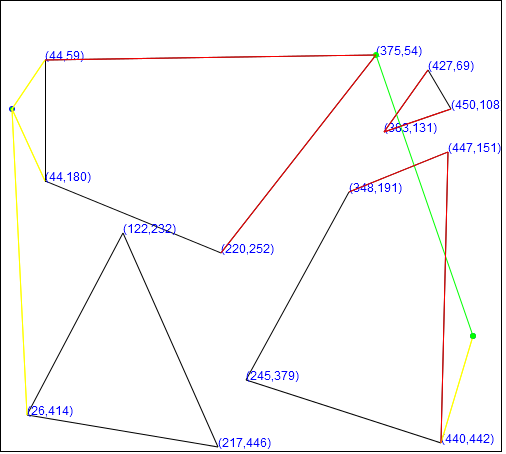
\includegraphics[scale=0.5]{img/visgraph.png}
	\end{center}	
\end{figure}
\newpage
Durante a execução do Algoritmo de Dijkstra, o grafo de visibilidade está pintado em amarelo, o ponto vermelho grande é o vértice atual (que possui as arestas pintadas em vermelho), os pontos azuis estão na fila de prioridade e os pontos rosas já foram analisados. A distância até cada ponto está escrita ao lado de cada ponto.

\begin{figure}[!htp]
	\begin{center}
		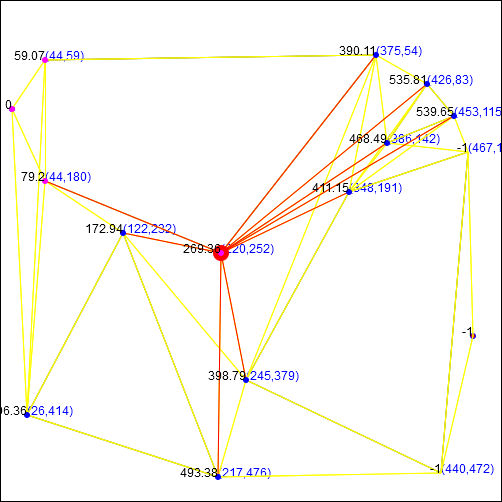
\includegraphics[scale=0.5]{img/dijkstra.png}
	\end{center}	
\end{figure}

\newpage

O resultado final do algoritmo é mostrado em vermelho.

\begin{figure}[!htp]
	\begin{center}
		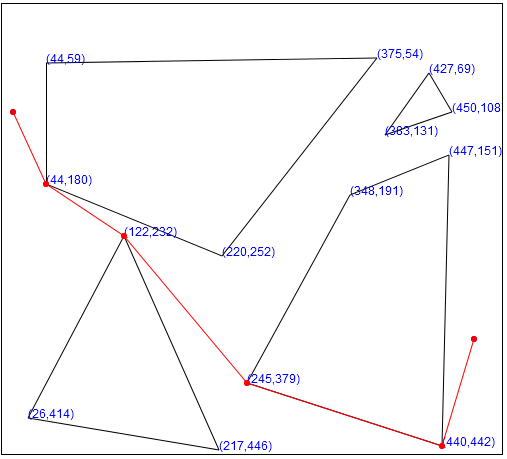
\includegraphics[scale=0.5]{img/final.png}
	\end{center}	
\end{figure}


\subsection{Complexidade}

Por falta de tempo, não consegui implementar as estruturas de dados descritas no livro. Por esta razão, a implementação que fiz leva tempo $O(n^3)$, principalmente por não manter o estado da linha de varredura em uma árvore binária balanceada.


\end{document}
